% Options for packages loaded elsewhere
\PassOptionsToPackage{unicode}{hyperref}
\PassOptionsToPackage{hyphens}{url}
%
\documentclass[
  man]{apa6}
\usepackage{amsmath,amssymb}
\usepackage{lmodern}
\usepackage{ifxetex,ifluatex}
\ifnum 0\ifxetex 1\fi\ifluatex 1\fi=0 % if pdftex
  \usepackage[T1]{fontenc}
  \usepackage[utf8]{inputenc}
  \usepackage{textcomp} % provide euro and other symbols
\else % if luatex or xetex
  \usepackage{unicode-math}
  \defaultfontfeatures{Scale=MatchLowercase}
  \defaultfontfeatures[\rmfamily]{Ligatures=TeX,Scale=1}
\fi
% Use upquote if available, for straight quotes in verbatim environments
\IfFileExists{upquote.sty}{\usepackage{upquote}}{}
\IfFileExists{microtype.sty}{% use microtype if available
  \usepackage[]{microtype}
  \UseMicrotypeSet[protrusion]{basicmath} % disable protrusion for tt fonts
}{}
\makeatletter
\@ifundefined{KOMAClassName}{% if non-KOMA class
  \IfFileExists{parskip.sty}{%
    \usepackage{parskip}
  }{% else
    \setlength{\parindent}{0pt}
    \setlength{\parskip}{6pt plus 2pt minus 1pt}}
}{% if KOMA class
  \KOMAoptions{parskip=half}}
\makeatother
\usepackage{xcolor}
\IfFileExists{xurl.sty}{\usepackage{xurl}}{} % add URL line breaks if available
\IfFileExists{bookmark.sty}{\usepackage{bookmark}}{\usepackage{hyperref}}
\hypersetup{
  pdftitle={Netflix case study: Genre vs decade},
  pdfkeywords={keywords},
  hidelinks,
  pdfcreator={LaTeX via pandoc}}
\urlstyle{same} % disable monospaced font for URLs
\usepackage{graphicx}
\makeatletter
\def\maxwidth{\ifdim\Gin@nat@width>\linewidth\linewidth\else\Gin@nat@width\fi}
\def\maxheight{\ifdim\Gin@nat@height>\textheight\textheight\else\Gin@nat@height\fi}
\makeatother
% Scale images if necessary, so that they will not overflow the page
% margins by default, and it is still possible to overwrite the defaults
% using explicit options in \includegraphics[width, height, ...]{}
\setkeys{Gin}{width=\maxwidth,height=\maxheight,keepaspectratio}
% Set default figure placement to htbp
\makeatletter
\def\fps@figure{htbp}
\makeatother
\setlength{\emergencystretch}{3em} % prevent overfull lines
\providecommand{\tightlist}{%
  \setlength{\itemsep}{0pt}\setlength{\parskip}{0pt}}
\setcounter{secnumdepth}{-\maxdimen} % remove section numbering
\usepackage{booktabs}
\usepackage{longtable}
\usepackage{array}
\usepackage{multirow}
\usepackage{wrapfig}
\usepackage{float}
\usepackage{colortbl}
\usepackage{pdflscape}
\usepackage{tabu}
\usepackage{threeparttable}
\usepackage{threeparttablex}
\usepackage[normalem]{ulem}
\usepackage{makecell}
\usepackage{xcolor}
\ifluatex
  \usepackage{selnolig}  % disable illegal ligatures
\fi
\newlength{\cslhangindent}
\setlength{\cslhangindent}{1.5em}
\newlength{\csllabelwidth}
\setlength{\csllabelwidth}{3em}
\newenvironment{CSLReferences}[2] % #1 hanging-ident, #2 entry spacing
 {% don't indent paragraphs
  \setlength{\parindent}{0pt}
  % turn on hanging indent if param 1 is 1
  \ifodd #1 \everypar{\setlength{\hangindent}{\cslhangindent}}\ignorespaces\fi
  % set entry spacing
  \ifnum #2 > 0
  \setlength{\parskip}{#2\baselineskip}
  \fi
 }%
 {}
\usepackage{calc}
\newcommand{\CSLBlock}[1]{#1\hfill\break}
\newcommand{\CSLLeftMargin}[1]{\parbox[t]{\csllabelwidth}{#1}}
\newcommand{\CSLRightInline}[1]{\parbox[t]{\linewidth - \csllabelwidth}{#1}\break}
\newcommand{\CSLIndent}[1]{\hspace{\cslhangindent}#1}

\title{Netflix case study: Genre vs decade}
\author{true}
\date{}

\begin{document}
\maketitle

{
\setcounter{tocdepth}{3}
\tableofcontents
}
\hypertarget{citations-in-papaja-detele-appropriately-later}{%
\section{Citations in papaja, detele appropriately
later}\label{citations-in-papaja-detele-appropriately-later}}

Add the bibtex entry in the .bib file. You can find the entries in
Google scholar, but double check since it is not always correct.

Call the citations in the text:

Citation within parentheses (Aust and Barth 2020)

Multiple citations (Aust and Barth 2020; R Core Team 2021)

In-text citations Aust and Barth (2020)

Year only (2021)

Only if your citation appears in the text it will also show up in the
Reference list. Don't manually modify the Reference list.

\hypertarget{executive-summary}{%
\subsection{Executive Summary}\label{executive-summary}}

(150 words) -- 0.3 POINTS Summarize the report. Write this as the very
last thing.

What is the main topic you are addressing?

what are your research questions and hypotheses?

what are your results and the main conclusion?

\hypertarget{introduction}{%
\subsection{Introduction}\label{introduction}}

\hypertarget{main-topic}{%
\subsubsection{Main topic}\label{main-topic}}

In this paper, we are going to study the presence of social networks
within a movie streaming platform. We're focusing on the structure of
links among a group of social players, which consist of users watching
and rating movies on Netflix.\\
Users of Netflix's movie recommendation algorithms are frequently given
specific questions about their interests for certain items (which they
provide by liking or disliking them, for example). These choices are
then immediately integrated into the underlying learning system for
future suggestions. If a recommender system starts promoting unwanted
products after incorporating new preferences, the user may try to steer
the system in the future by correcting it or supplying alternate
preference information.

\hypertarget{importance}{%
\subsubsection{Importance}\label{importance}}

It is important to study the presence of these socials networks because
this could potentially improve the recommender engine that this
currently in place. For example, if you know that a user is likely to
like a movie that other users with the same ``liking profile'' also
like, you can recommend that movie to the user. When these connections
are studied thoroughly, you could have a high probability that the
recommendation is successful. This could have a large impact on a movie
streaming platform.

\hypertarget{existing-studies}{%
\subsubsection{Existing studies}\label{existing-studies}}

In this paper, we will be looking into the Netflix Price Dataset. In
2006 Netflix decided to start a competition with a grand prize of 1
million US dollars. The goal of the competition was to create a
collaborative filtering algorithm to predict user ratings for films,
based on previous ratings without any other information about the users
or films. In order to win you had to at least improve on Netflix's own
algorithm by 10\%. During the competition a lot of literature has
emerged about the dataset and the competition. (Bell and Koren 2007;
Takács et al. 2008; Narayanan and Shmatikov 2006)

However, no papers or any other literature can be found on network
analysis on this dataset. We like to fill this gap in the literature by
analysing the network and network structure that arises from the subset
of the data that we will use. (Guillory and Bilmes 2011) developed an
active movie recommendation system for Netflix. They found that a
recommender system should not constantly ask questions to a user,
because those reduces the user's mental image of how the recommendation
system learns, prompting some participants to ``lose track of what they
were teaching.'' According to Amershi et al. (2014), this was because
users are not always eager to act as simple oracles (repeatedly telling
the recommendation system whether they like something or not). This is
interesting to take into account for our research, because this would
mean that a social network within a movie recommendation system can
never be fully exposed.

\hypertarget{questions-and-hypotheses}{%
\subsubsection{Questions and
hypotheses}\label{questions-and-hypotheses}}

In this dataset, we can easily see connections between users and movies,
but not between just the users or just the movies. At least not, when we
do not include one or the other.

\hypertarget{methodology}{%
\subsection{Methodology}\label{methodology}}

\hypertarget{dataset}{%
\subsubsection{Dataset}\label{dataset}}

During this study, the data that was shared by Netflix during the
Netflix Prize open competition is used. The competition was about
developing the best algorithm to predict user ratings for content on
Netflix. The contest was started in order to improve their recommender
system.

The data consisted of movies and account holders on Netflix who rated
the movies on a 5 point scale. Also, the date the rating that was given
and the year of the movie release are included in the dataset. Data was
collected between October 1998 and December 2005 and the data consists
of all ratings that were given during this period. (REF: KAGGLE) The
initial dataset contains about 100 million ratings from over 480k users
on almost 18k movies. (REF: Matrix Factorization and Neighbor Based
Algorithms for the Netflix Prize Problem)

In order to answer research questions about liking behaviour of
customers on streaming platforms (such as Netflix) this dataset provides
us with a great opportunity. The dataset contains a unusual amount of
real, user generated data. Datasets with similar types of data usually
contain a lot less data and the large dataset is thus very useful in
order to answer research questions about liking behaviour. (REF: Matrix
Factorization and Neighbor Based Algorithms for the Netflix Prize
Problem)

As stated in the initial distribution of the data, Netflix can and will
not guarantee the correctness of the data. As no perfect documentation
of the data collection exists, this can cause inaccuracies in the
results. Also, Netflix uses algorithms that determine what users see and
this effect can influence the results of this research. We could
interpret the effect of the algorithm as a effect caused by user
behaviour.

\hypertarget{descriptives}{%
\paragraph{Descriptives}\label{descriptives}}

\begin{table}
\centering
\begin{tabular}{l|l|l|l|l|l}
\hline
  &       X &   CustomerID &     Rating &     Date &    Movie\_Id\\
\hline
 & Min.   :     5025 & Min.   :     79 & Min.   :1.000 & Length:864610 & Min.   :    7\\
\hline
 & 1st Qu.: 26370543 & 1st Qu.: 671925 & 1st Qu.:3.000 & Class :character & 1st Qu.: 4906\\
\hline
 & Median : 52361182 & Median :1305946 & Median :3.000 & Mode  :character & Median : 9509\\
\hline
 & Mean   : 51568441 & Mean   :1313868 & Mean   :3.362 & NA & Mean   : 9301\\
\hline
 & 3rd Qu.: 77757849 & 3rd Qu.:1963714 & 3rd Qu.:4.000 & NA & 3rd Qu.:14149\\
\hline
 & Max.   :100488407 & Max.   :2649296 & Max.   :5.000 & NA & Max.   :17765\\
\hline
\end{tabular}
\end{table}

Looking at the average Rating of the users in the data, the avarage
rating they gave was about a \(3,36\).

\begin{table}
\centering
\begin{tabular}{l|r|r|r|r|r}
\hline
  & mean & sd & min & max & n\\
\hline
Rating & 3.362346 & 1.114827 & 1 & 5 & 864610\\
\hline
\end{tabular}
\end{table}

Looking at the histogram of the amound of ratings given on a certain
date we can see that a peak in ratings exists always in the middle of
the week (around wednesday/thursday). Looking at the distribution of the
ratings over time we don't see great differences. Over time, people give
consistent ratings.

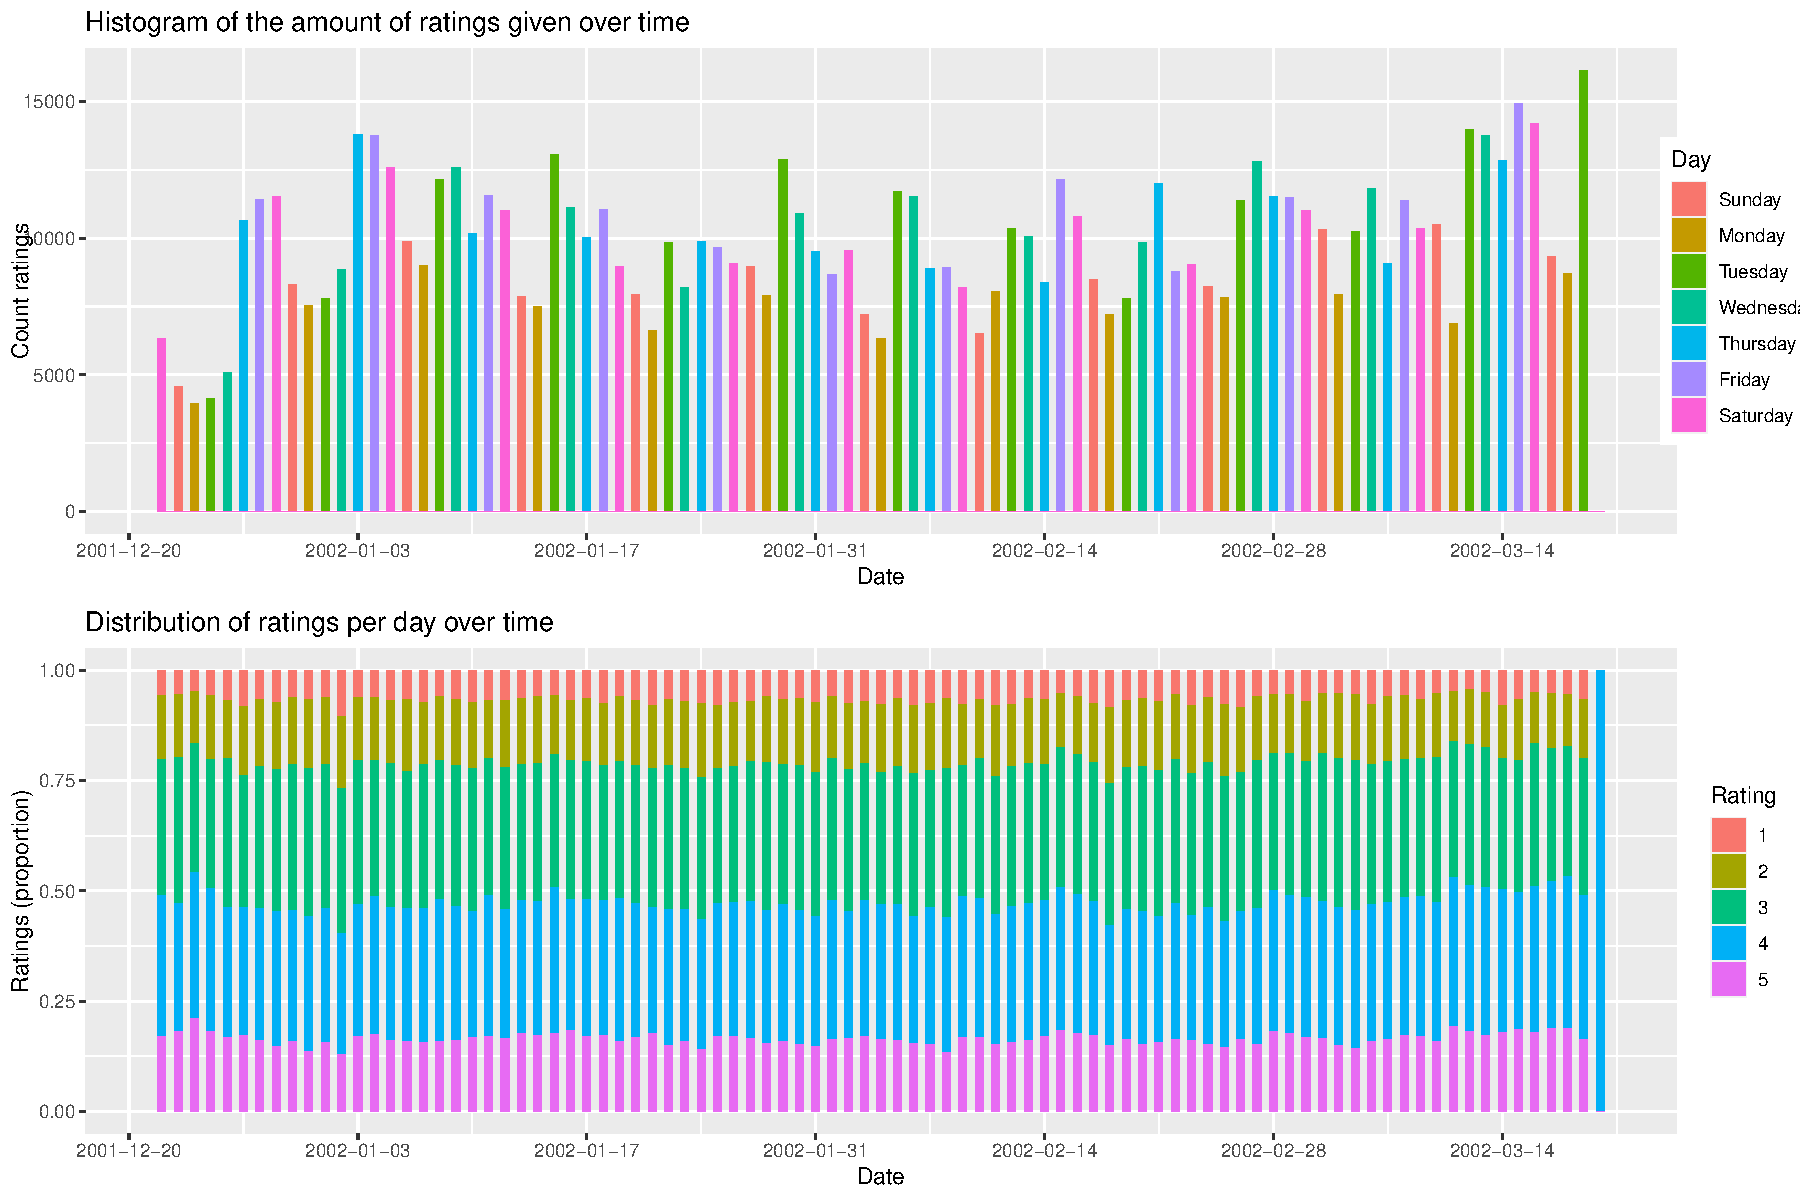
\includegraphics{tawab_backup_report_files/figure-latex/unnamed-chunk-5-1.pdf}

\hypertarget{data-analysis-research-rationale}{%
\subsubsection{Data analysis (Research
Rationale)}\label{data-analysis-research-rationale}}

(about 500 words) -- 1 POINTS * Why are these two methods suitable for
your data?

\begin{itemize}
\item
  Why are these two methods suitable for your research questions?
\item
  Are there other methods to address these questions? If yes, why are
  the methods you chose better for this case?
\end{itemize}

\hypertarget{results}{%
\subsection{Results}\label{results}}

(about 2000 words)

Wat voor tekst moeten wij hier typen??

\hypertarget{qap-model}{%
\subsubsection{QAP Model}\label{qap-model}}

(about 1000 words) -- 2.5 POINTS

\hypertarget{constructing-data-and-the-model}{%
\paragraph{Constructing data and the
model}\label{constructing-data-and-the-model}}

During preprocessing of the data, an interesting artifact was
encountered; When users were removed from the dataset that either liked
or disliked a movie, it was clearly shown that it occurred much more
often that user gave a 4/5 star rating to a movie than a 1/2 star
rating. This is interesting to keep in mind, as this might pose a
potential bias in the dataset.

To give a weight to the edges in terms of importance, we calculate the
weight according to a formula: \$weight =
\frac{no. of mutual liked movies}{max(no. of liked movies)} \$

\hypertarget{results-1}{%
\paragraph{Results}\label{results-1}}

\begin{itemize}
\tightlist
\item
  Present your results appropriately (plots, tables\ldots) and discuss
  your findings in plain English
\end{itemize}

\hypertarget{findings-in-relation-to-hypothesis}{%
\paragraph{Findings in relation to
hypothesis}\label{findings-in-relation-to-hypothesis}}

\begin{itemize}
\tightlist
\item
  Discuss the meaning of your findings in relation to your hypothesis.
  (half of the points evaluated in this other part)
\end{itemize}

\begin{tabular}{l|l|l}
\hline
age & gender & eyes\_col\\
\hline
7 & M & BLUE\\
\hline
8 & F & BROWN\\
\hline
8 & M & GREEN\\
\hline
7 & F & PINK\\
\hline
\end{tabular}

\hypertarget{ergm}{%
\subsubsection{ERGM}\label{ergm}}

(about 1000) -- 2.5 POINTS

In order to answer this research question, an ERGM model has been used.
The netwerk created consists of movies as nodes. Two movies get an
undirected edge if at least one user exists that has watched and liked
both movies. An important assumption that is made is that a user liked a
movie if the user has given a rating of at least four out of five. Next,
in order to assess the influence of the release date, the decade of the
release date is used. Furthermore, only the main genre of the movies
have been used to assess the influence of two movies being watched by
one user.

Homophily is hypothesized for genre and decade. Two movies with the same
genre are more likely to have an edge and two movies from the same
release decade are more likely to have an edge. Furthermore, the
likeliness of an edge is even bigger when a movie has both the same
genre and is from the same decade.

\hypertarget{the-genre}{%
\paragraph{The Genre}\label{the-genre}}

To start off, the effect of genre on the likelihood of an edge between
movies will be explored.

\hypertarget{ergm-model-results}{%
\paragraph{ERGM Model results}\label{ergm-model-results}}

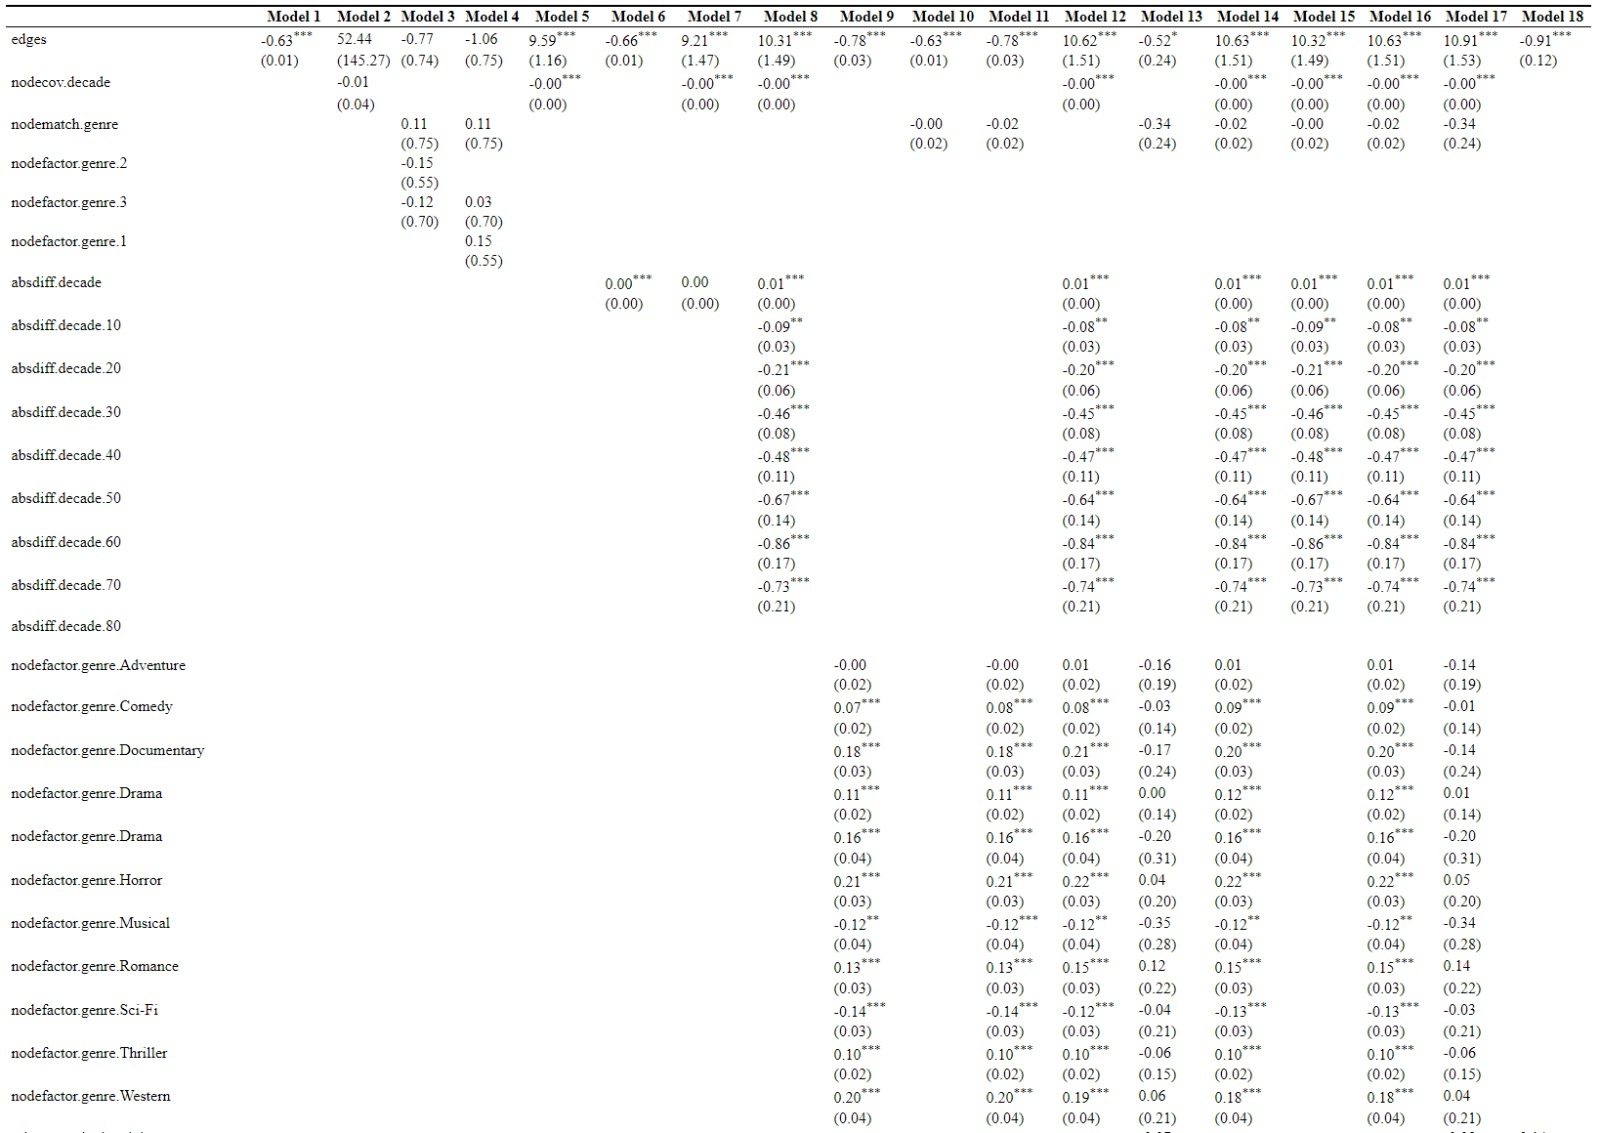
\includegraphics{ergm_images/model_result1.jpeg}
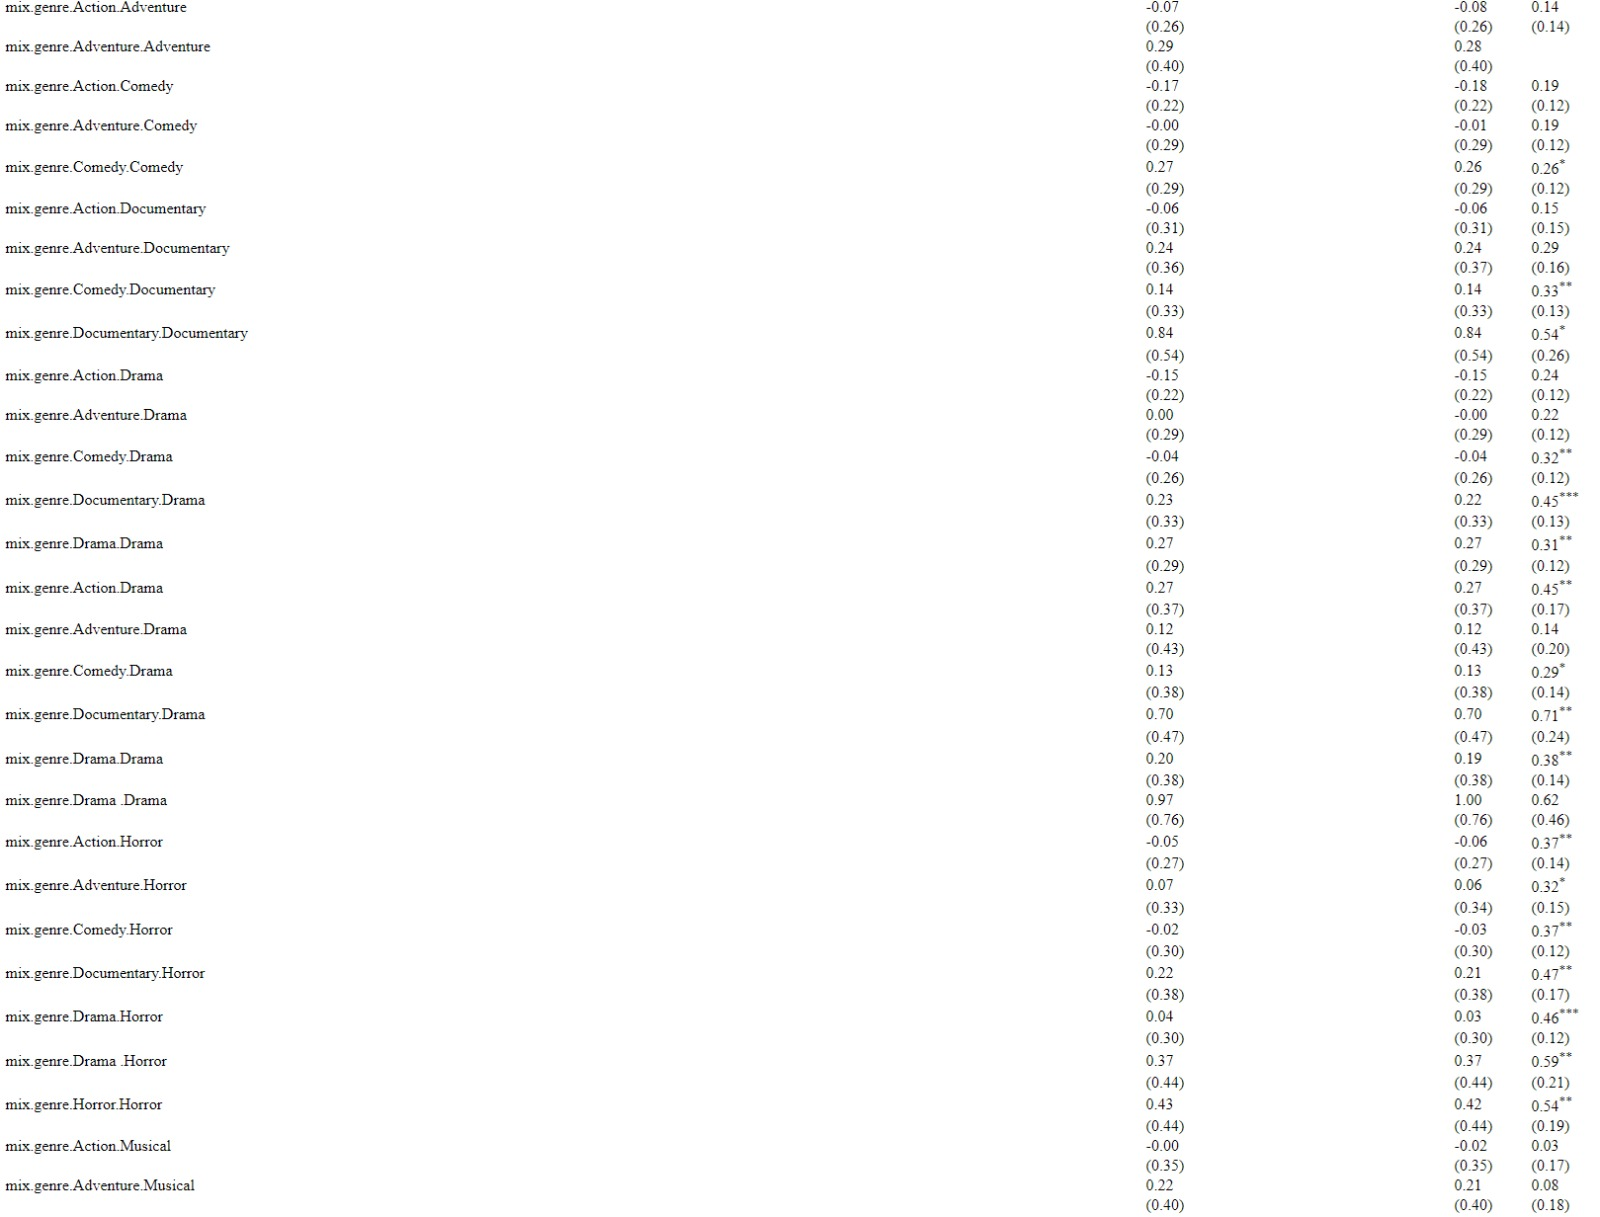
\includegraphics{ergm_images/model_result2.jpeg}
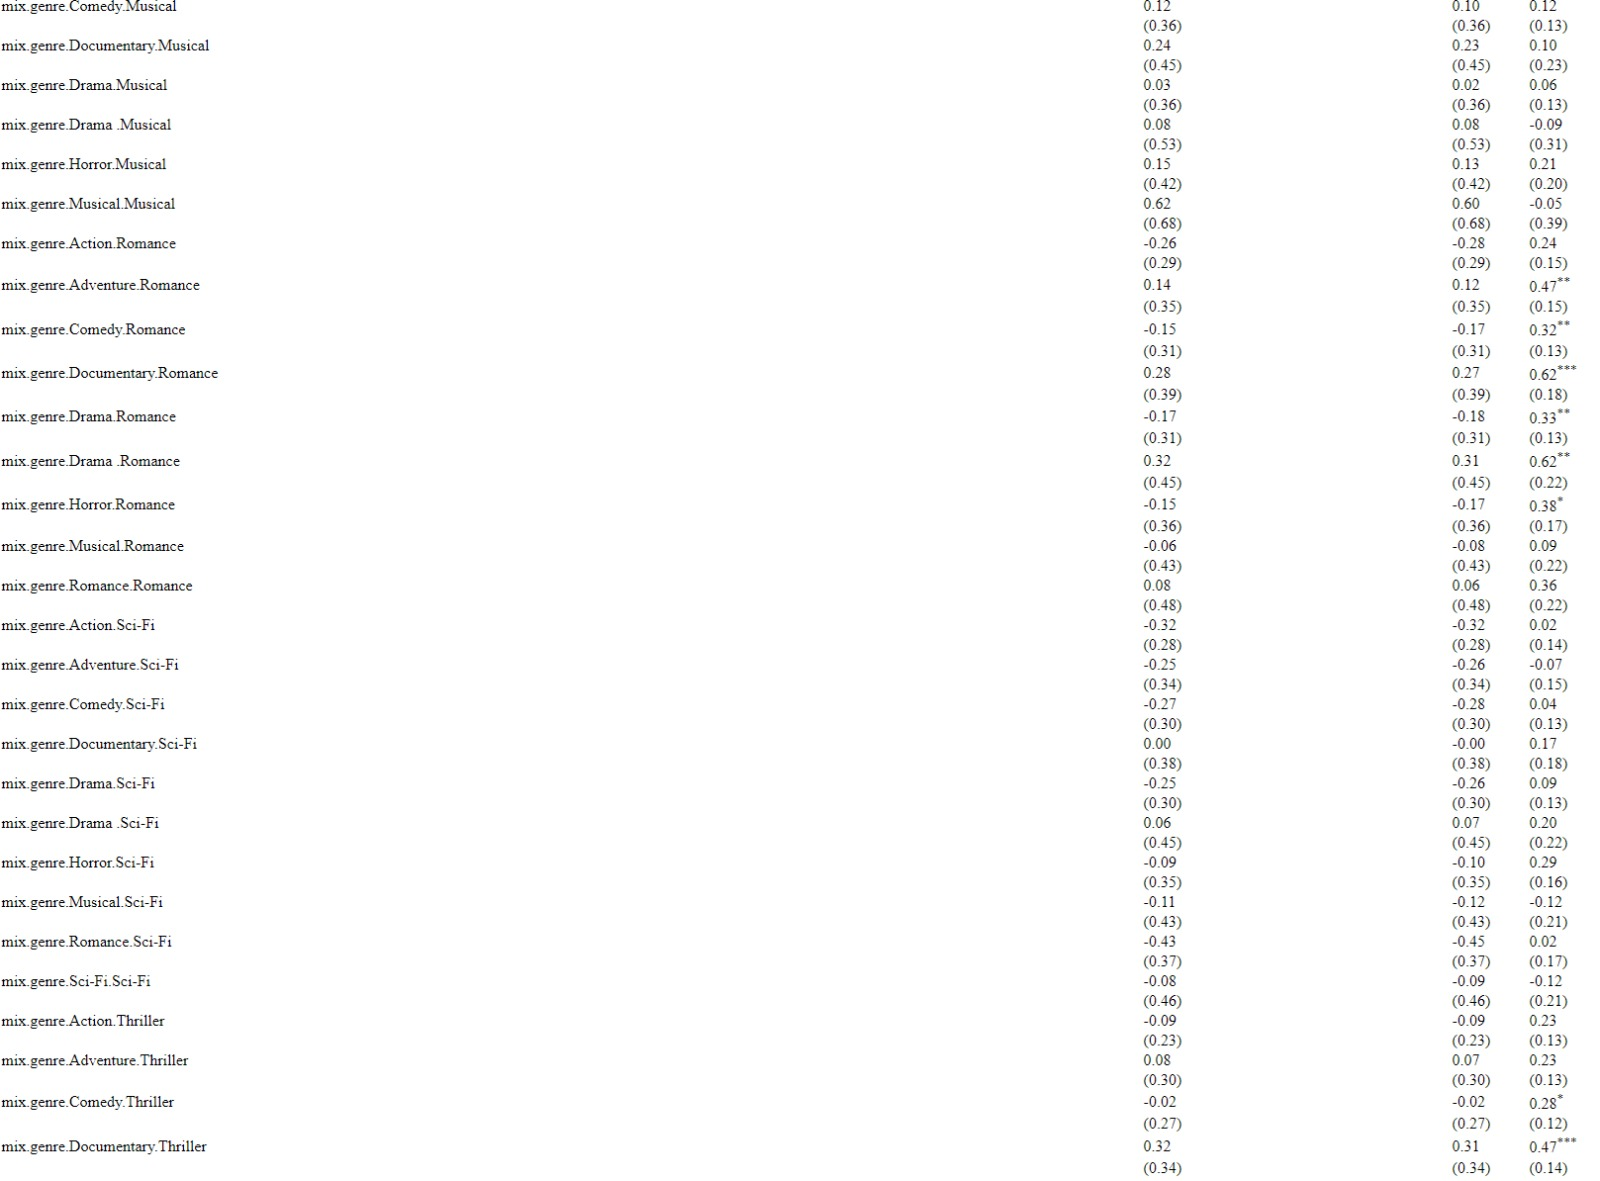
\includegraphics{ergm_images/model_result3.jpeg}
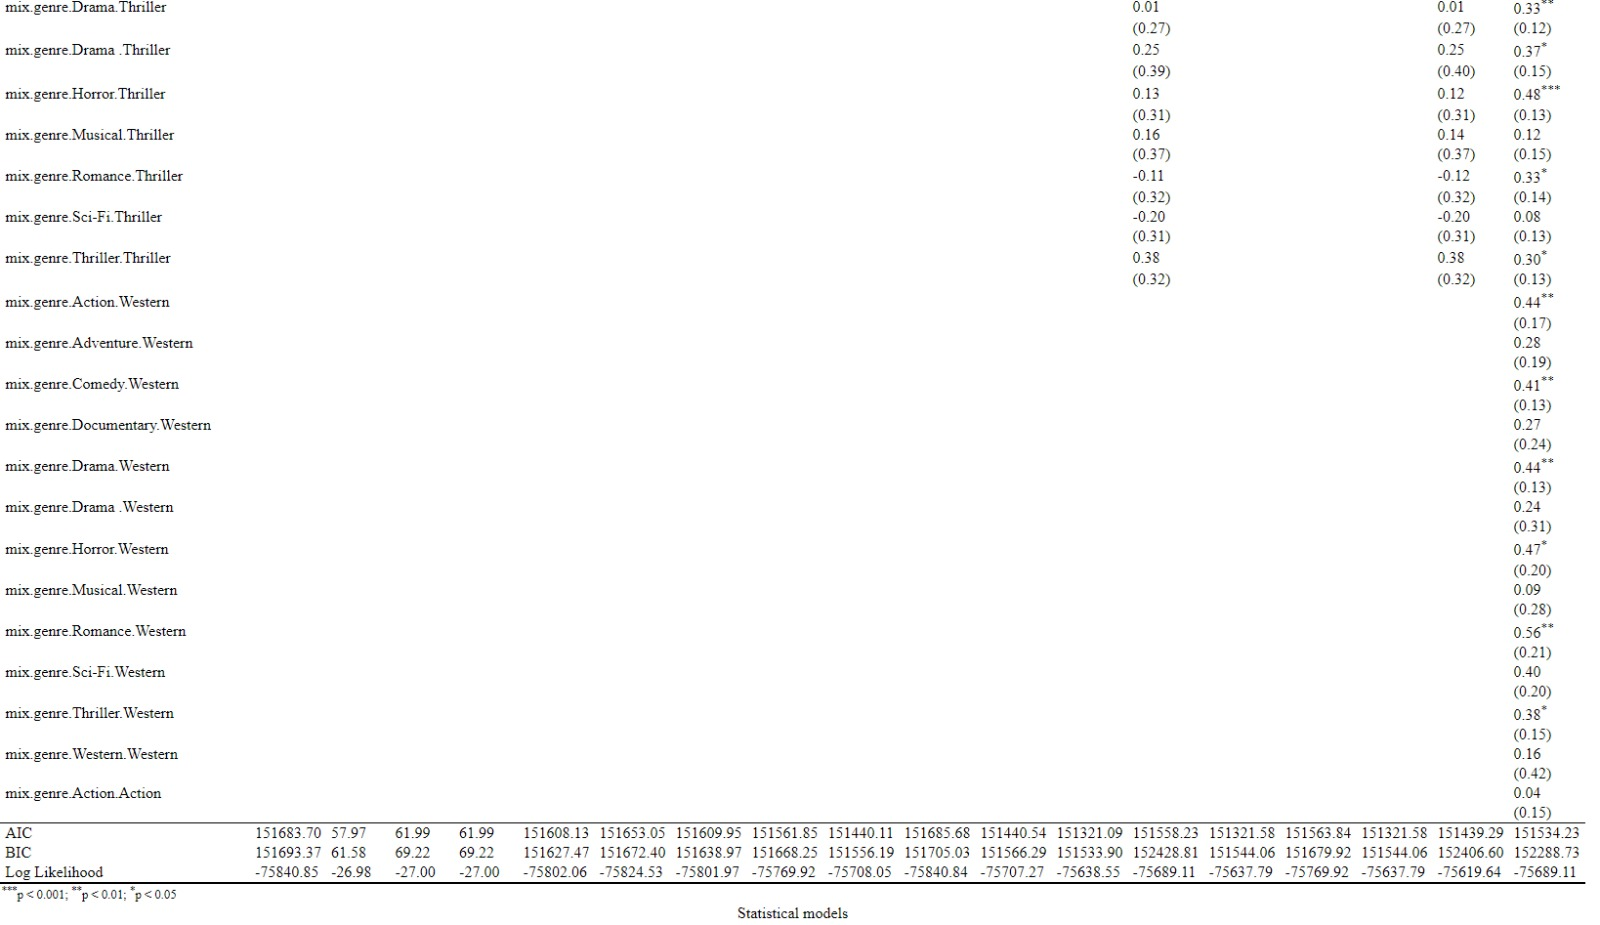
\includegraphics{ergm_images/model_result4.jpeg}

\begin{itemize}
\item
  Present your results appropriately (plots, tables\ldots) and discuss
  your findings in plain English
\item
  Discuss the meaning of your findings in relation to your hypothesis.
  (half of the points evaluated in this other part)
\end{itemize}

Option to showcase a model:

\begin{tabular}{l|l|l}
\hline
 & Model 1 & Model 2\\
\hline
(Intercept) & 5.03 *** & \\
\hline
 & (0.22) & \\
\hline
groupTrt & -0.37 & 4.66 ***\\
\hline
 & (0.31) & (0.22)\\
\hline
groupCtl &  & 5.03 ***\\
\hline
 &  & (0.22)\\
\hline
R\textasciicircum{}2 & 0.07 & 0.98\\
\hline
Adj. R\textasciicircum{}2 & 0.02 & 0.98\\
\hline
Num. obs. & 20 & 20\\
\hline
\end{tabular}

Option 3

\begin{verbatim}
## Model: bars denote 0.5 (inner) resp. 0.95 (outer) confidence intervals (computed from standard errors).
\end{verbatim}

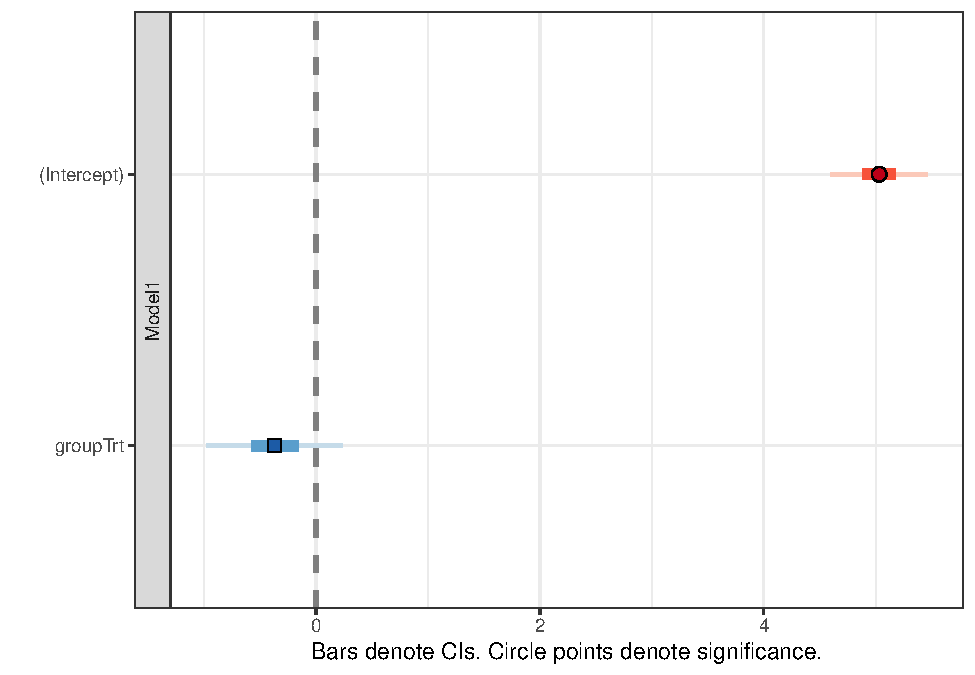
\includegraphics{tawab_backup_report_files/figure-latex/model 3-1.pdf}

Option 4

\begin{verbatim}
## Models: bars denote 0.5 (inner) resp. 0.95 (outer) confidence intervals (computed from standard errors).
\end{verbatim}

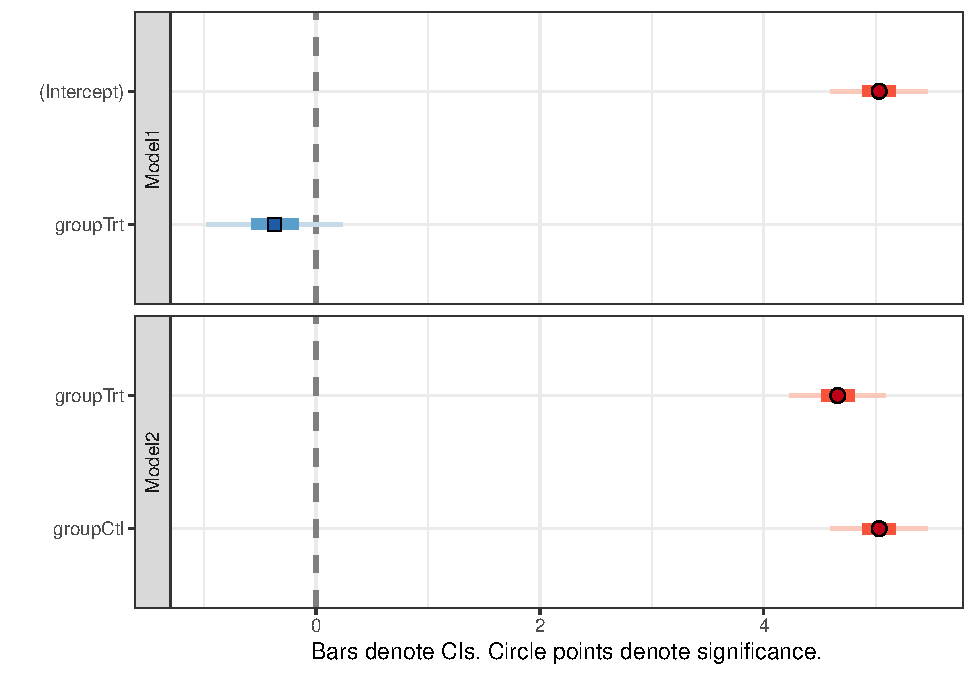
\includegraphics{tawab_backup_report_files/figure-latex/model 4-1.pdf}

\hypertarget{conclusion}{%
\subsection{Conclusion}\label{conclusion}}

(about 350 words) -- 0.7 POINTS What were your topic and research
questions again? (1 sentence)

What did you learn from the two analysis you run? *** most important
point to address 0.5 POINTS here

Who benefits from your findings?

What does remain an open problem?

Can you give suggestions for future work in this area?

\newpage

\hypertarget{references}{%
\section{References}\label{references}}

\begingroup
\setlength{\parindent}{-0.5in}
\setlength{\leftskip}{0.5in}

\hypertarget{refs}{}
\begin{CSLReferences}{1}{0}
\leavevmode\hypertarget{ref-amershi2014power}{}%
Amershi, Saleema, Maya Cakmak, William Bradley Knox, and Todd Kulesza.
2014. {``Power to the People: The Role of Humans in Interactive Machine
Learning.''} \emph{Ai Magazine} 35 (4): 105--20.

\leavevmode\hypertarget{ref-R-papaja}{}%
Aust, Frederik, and Marius Barth. 2020. \emph{{papaja}: {Create} {APA}
Manuscripts with {R Markdown}}. \url{https://github.com/crsh/papaja}.

\leavevmode\hypertarget{ref-bell2007lessons}{}%
Bell, Robert M, and Yehuda Koren. 2007. {``Lessons from the Netflix
Prize Challenge.''} \emph{Acm Sigkdd Explorations Newsletter} 9 (2):
75--79.

\leavevmode\hypertarget{ref-guillory2011simultaneous}{}%
Guillory, Andrew, and Jeff A Bilmes. 2011. {``Simultaneous Learning and
Covering with Adversarial Noise.''} In \emph{ICML}.

\leavevmode\hypertarget{ref-narayanan2006break}{}%
Narayanan, Arvind, and Vitaly Shmatikov. 2006. {``How to Break Anonymity
of the Netflix Prize Dataset.''} \emph{arXiv Preprint Cs/0610105}.

\leavevmode\hypertarget{ref-R-base}{}%
R Core Team. 2021. \emph{R: A Language and Environment for Statistical
Computing}. Vienna, Austria: R Foundation for Statistical Computing.
\url{https://www.R-project.org/}.

\leavevmode\hypertarget{ref-takacs2008matrix}{}%
Takács, Gábor, István Pilászy, Bottyán Németh, and Domonkos Tikk. 2008.
{``Matrix Factorization and Neighbor Based Algorithms for the Netflix
Prize Problem.''} In \emph{Proceedings of the 2008 ACM Conference on
Recommender Systems}, 267--74.

\end{CSLReferences}

\endgroup

\end{document}
